\documentclass[12pt,oneside]{udthesis}\usepackage[]{graphicx}\usepackage[]{color}
% maxwidth is the original width if it is less than linewidth
% otherwise use linewidth (to make sure the graphics do not exceed the margin)
\makeatletter
\def\maxwidth{ %
  \ifdim\Gin@nat@width>\linewidth
    \linewidth
  \else
    \Gin@nat@width
  \fi
}
\makeatother

\definecolor{fgcolor}{rgb}{0.345, 0.345, 0.345}
\newcommand{\hlnum}[1]{\textcolor[rgb]{0.686,0.059,0.569}{#1}}%
\newcommand{\hlstr}[1]{\textcolor[rgb]{0.192,0.494,0.8}{#1}}%
\newcommand{\hlcom}[1]{\textcolor[rgb]{0.678,0.584,0.686}{\textit{#1}}}%
\newcommand{\hlopt}[1]{\textcolor[rgb]{0,0,0}{#1}}%
\newcommand{\hlstd}[1]{\textcolor[rgb]{0.345,0.345,0.345}{#1}}%
\newcommand{\hlkwa}[1]{\textcolor[rgb]{0.161,0.373,0.58}{\textbf{#1}}}%
\newcommand{\hlkwb}[1]{\textcolor[rgb]{0.69,0.353,0.396}{#1}}%
\newcommand{\hlkwc}[1]{\textcolor[rgb]{0.333,0.667,0.333}{#1}}%
\newcommand{\hlkwd}[1]{\textcolor[rgb]{0.737,0.353,0.396}{\textbf{#1}}}%
\let\hlipl\hlkwb

\usepackage{framed}
\makeatletter
\newenvironment{kframe}{%
 \def\at@end@of@kframe{}%
 \ifinner\ifhmode%
  \def\at@end@of@kframe{\end{minipage}}%
  \begin{minipage}{\columnwidth}%
 \fi\fi%
 \def\FrameCommand##1{\hskip\@totalleftmargin \hskip-\fboxsep
 \colorbox{shadecolor}{##1}\hskip-\fboxsep
     % There is no \\@totalrightmargin, so:
     \hskip-\linewidth \hskip-\@totalleftmargin \hskip\columnwidth}%
 \MakeFramed {\advance\hsize-\width
   \@totalleftmargin\z@ \linewidth\hsize
   \@setminipage}}%
 {\par\unskip\endMakeFramed%
 \at@end@of@kframe}
\makeatother

\definecolor{shadecolor}{rgb}{.97, .97, .97}
\definecolor{messagecolor}{rgb}{0, 0, 0}
\definecolor{warningcolor}{rgb}{1, 0, 1}
\definecolor{errorcolor}{rgb}{1, 0, 0}
\newenvironment{knitrout}{}{} % an empty environment to be redefined in TeX

\usepackage{alltt}

%----------------------------------------------------------------------------------------
%	Atributes Settings
%----------------------------------------------------------------------------------------
% About your study degree programme
\def \study{ITM} % possible options: ITM, SWD, MSD, IRM, IMS

% More about you and your thesis:
\def \Title{TESIS}
\def \title{PRA TESIS}
\def \subtitle{Pengaruh Fitur Binaan Terhadap Aktivitas di Jalan Pinggir Laut}
\def \yourName{Muhammad Uliah Shafar}
\def \yourIdentifier{21020119420029}
\def \yourPlace{<place>}
\def \submissionDate{<date>}  % month year. e.g. June 2017
\DTMsavedate{tanggalberita}{2021-01-31} %tanggal sidang
\DTMsavetime{waktuberita}{24:60:60} %waktu sidang
\def \hariBerita{<day>} %hari sidang
\def \yourAdvisor{<firstname lastname>}
\def \yourNipAdvisor{<xxxxxxxxx xxxxxxxx>}
\def \yourSecAdvisor{<firstname lastname>}
\def \yourNipSecAdvisor{<xxxxxxxxx xxxxxxxx>}
%\def \thisDocumentIsA{Thesis} % possible options:
                     % Thesis  .... for Master's Thesis   / Masterarbeit
                     % Thesis  .... for Bachelor's Thesis / Bachelorarbeit
                     % Seminar .... for Seminar Work      / Seminararbeit
                     % Project .... for Project Work      / Projektarbeit

% ITM/SWD/IRM: you could possibly write in German.
%\def \yourLanguage{english} % possible options: german, english
\IfFileExists{upquote.sty}{\usepackage{upquote}}{}
\begin{document}


%----------------------------------------------------------
% Front Matter
%
%----------------------------------------------------------
\subfile{../subfiles/01_titlepage.tex}
\subfile{../subfiles/01titlepage.tex}

\pagenumbering{roman}
\subfile{../subfiles/02declaration.tex}
\subfile{../subfiles/03validation.tex}
\subfile{../subfiles/04agreement.tex}
\subfile{../subfiles/05private.tex}
\subfile{../subfiles/06abstrak.tex}
\subfile{../subfiles/07abstract.tex}
\subfile{../subfiles/08acknowledge.tex}

%----------------------------------------------------------
% Table Of Content
%
%----------------------------------------------------------
%\tableofcontents
\clearpage
\addcontentsline{toc}{chapter}{\listfigurename}
\listoffigures
\clearpage
\addcontentsline{toc}{chapter}{\listtablename}
\listoftables

%----------------------------------------------------------
% Body Matter
%
%----------------------------------------------------------
\clearpage
\pagenumbering{arabic}
\subfile{../subfiles/introduction.tex}
\subfile{../subfiles/literature.tex}
\subfile{../subfiles/method.tex}

% !Rnw root = thesis.Rnw
% Child with Latex code only - Work as a subfiles:

%---------------------------------------------------

%---------------------------------------------------


%---------------------------------------------------

%------------------------------------------------------

%------------------------------------------------------



\newcommand{\pieChartFig}
{\begin{figure}[h]
\centering

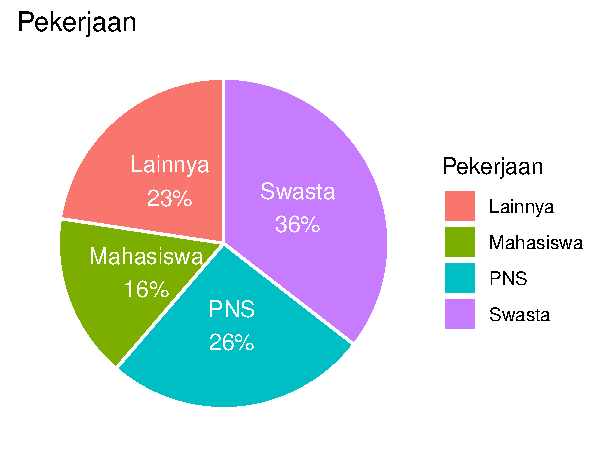
\includegraphics[width=\maxwidth]{../figures/stats2-1} 
\caption{Pie Chart Pekerjaan}
\label{pieChartFig}\end{figure}
}



\newcommand{\tabRegresi}{
% latex table generated in R 4.0.3 by xtable 1.8-4 package
% Tue Feb 16 17:36:46 2021
\begin{table}[ht]
\centering
\begin{tabular}{lrrrrr}
  \hline
 & Df & Sum Sq & Mean Sq & F value & Pr($>$F) \\ 
  \hline
data2\$total\_fit & 1.000 & 96.998 & 96.998 & 3.679 & 0.065 \\ 
  Residuals & 29.000 & 764.551 & 26.364 &  &  \\ 
   \hline
\end{tabular}
\caption{Regresi Linear} 
\label{tabRegresi}
\end{table}
}

%-------------------------------------------------

\section{ Knitr child Documents}
You should note that using knitr package you can easily incorporate difference kinds of files into a project.

\tabRegresi
\pieChartFig
\subfile{../subfiles/conclusion.tex}

%----------------------------------------------------------
% End Matter
%
%----------------------------------------------------------
\subfile{../subfiles/09beritaacara.tex}
\subfile{../subfiles/10biography.tex}






%----------------------------------------------------------------------------------------
%	BIBLIOGRAPHY
\bibliographystyle{apalike}
\bibliography{biblio.bib}


\end{document}
